\chapter{Technical Background}
\section{Cryptographic Hash Functions}
A hash function is a function that maps arbitrary length data to a fixed length representation. An example of a (completely useless) hash function is the function that maps all inputs to the 0x00 byte. Useful hash functions often approximate a uniform distribution over the possible outputs for different inputs. If a hash function has an output length of one byte (256 possible outputs), and we feed in random strings to the hash function, it is desirable (for many use cases) if each of the 256 possibilities are approximately equally represented in the outputs. Hash functions with this property are useful in designing efficient algorithms and data structures (e.g. hash tables). However, the uniform distribution of outputs is not a sufficient property for making the hash function a secure cryptographic hash function. It is possible that the output of such a hash function reveals some information about the input. Let's construct an example of a hash function whose output reveals information about the input, we interpret the input message as an unsigned integer (with an arbitrary number of bits) and take the modulo of this integer and the number of possible outputs. Therefore the messages "0x00", "0x01", "0x02", ..., "0xFF" are all mapped to themselves, so we get a perfect uniform distribution for all one-byte messages. In fact, any message is just mapped to the least significant byte of the message, and therefore, the hash output tells us deterministically what the last byte of the message was. For hash functions used in cryptographic algorithms this is not acceptable; we need hash function where the hash digest (output) reveals nothing about the input message. Our insecure last-byte hash function is fast to compute (it's O(1), just take the last byte), but it turns out that cryptographically secure hash algorithms are more compute intensive because they ought to digest the entire input message (they are at least O(N)). One might not want to use a cryptographic hash function for non-cryptographic tasks (efficient lookup, hash tables etc.) because they may be more compute-intensive than non-cryptographic alternatives.
\section{AEAD}

[ ] AEAD in a nutshell

[ ] summary, how many available AEAD algorithms, exclusively use AEAD in TLS 1.3

[ ] description of the AEAD interface, requirements (unique nonce) and gaurantees over the values

[ ] Coordinating various devices using the same key requires some cleverness in nonce generation.

[ ] Using the same (nonce, key) pair results in the same key stream which is a "cryptographic disaster" (to quote RFC 7714 Section 6). See explanation in Section 9.1 of RFC3711.

\section{HKDF}

[ ] The HMAC-based Extract-and-Expand Key Derivation Functions (HKDF) described in RFC 5869 are used ubiquitously in the TLS 1.3 protocol for the derivation of various traffic encrpytion keys from the master secret derived in the handshake. Additionally the HKDF is proposed to be used for the ECH \var{accept\_confirmation} 8 bytes acceptance signal (see e.g. Section 7.2 of \cite{esni}). A Hashed Message Authentication Code (HMAC) (described by \cite{rfc2104}) is a pattern for performing message authentication based on cryptographic hash functions, and the authentication is secured with a secret key. The pattern works with any iterative cryptographic hash function. A HMAC scheme enables the calculation of the HMAC over data with a secret a key, and verification that the HMAC matches the data and secret key. A successful verificatoin of the HMAC implies that the data have not been tampered with (with high probability), and that the HMAC was calculated by someone who knows the secret key (with high probability). The precise security properties of the HMAC depends on the underlying cryptographic hash function.

[ ] The HKDF scheme is all about transforming some intput keying material (IKM) (some source of secret randomness/entropy) into a set of (yes multiple!) pseudorandom cryptographic keys. If the input keying material is already cryptographically strong and of the appropriate length then the HKDF-extract stage can be safely skipped and the IKM directly into a sequence of pseudorandom keys using the HKDF-expand function. It is possible, however, that the input keying material may be too long to be directly used in the HKDF-expand function, or it may not be cryptographically suitable, e.g. the Diffie-Hellman value $g^{xy}$ is not uniformly random and therefore not suitable as a PRK for the HKDF-Expand step. So long as the input keying material contains sufficient entropy (read randomness), we can extract an appropriately long, uniformly (pseudo)random key from the input keying material by applying the HKDF-extract function. For simplicity, when protocols use the extract-then-expand pattern, one can decide to always apply the HKDF-Extract stage, even if it is not always cryptographically necessary.

[ ] The HKDF-Extract function (the first step in the HKDF pattern) takes as input a salt (a non-secret random value) and the IKM to produce a pseudo-random key (PRK). The salt is optional and is set to all zeros if not provided to the function, but is highly recommended in RFC 5869 Section 3.1. Ideally the salt should be a random string with length equal to the length of the output of the underlying hash function used. The second step is the HKDF-Expand  function which takes as input a pseudorandom key, an optional information string (termed the label in TLS 1.3), and the desired length of the output, to produce the output keying material (OKM). The HKDF-Extract function is implemented as `HKDF-Extract(salt, IKM) = HMAC-Hash(salt, IKM)`, where the salt is being used as the key for the HMAC-Hash (but it does not have to be secret) and the IKM is the input message of the HMAC-Hash function. This means that the IKM can have arbitrary length. The OKM is generated recursively as `T(n) = HMAC-Hash(PRK, concatenate(T(n-1), info, n))`, but where `T(0)` is an empty string. This recursive pattern means that the OKM can be arbitrarily long. The info parameter in HKDF-Expand can be used to bind the OKM to particular contexts, e.g. in TLS 1.3 client-to-server and server-to-client encryption keys are generated with different info parameters. 

\section{HPKE}

\section{TLS 1.3}
\subsection{HRR}
With TLS 1.3 the server can (hopefully in an overwhelming majority of cases) generate the application traffic key after processing just one flight of messages from the client. This is possible because the client `guesses' a cipher suite and sends an appropriate \var{key\_share} in the ClientHello (in fact the client may send multiple \var{key\_share}s for multiple cipher suites to increase the probability that the server will support at least one of those cipher suites). However, if the client guesses wrong and sends a \var{key\_share} for a cipher suite not supported by the server, then the server should respond with a message that informs the client as to which cipher suites are supported. This subsequent message is called the HelloRetryRequest (HRR); 'Hello' because it is the first message sent by the server (if it is sent), and `RetryRequest' because the server is asking the client to rerty with a new ClientHello message (CH2) using different parameters.
[ ] The HRR message format is designed to look almost identical to the ServerHello (SH) message for compatibility with hardened TLS 1.2 middleboxes that fail to correctly ignore new message types (TODO: review this sentence).
From the perspective of a middlebox that is unaware of TLS 1.3 the HRR is treated just like a SH, but the client can distinguish between HRR and SH based on a special value in the \var{random} field of the message (which we would call the `ServerHello.random` if we interpreted the HRR as a SH).

The top-level structure of the HRR message is identical to the ServerHello message described in Listing. \ref{lst:server-hello-struct}, but the \var{random} in a HRR is in fact a fixed value, not a random value.

%\includecodescaleimage{lst:server-hello-struct}{ServerHello and HelloRetryRequest Structures}{The structure of the ServerHello message, which is the same as the structure of HelloRetryRequest, repeated from Section 4.1.3 of \cite{esni} using the presentation syntax defined by same.}{1}{figure/ServerHello-struct.pdf}


\begin{listing}
    \centering
    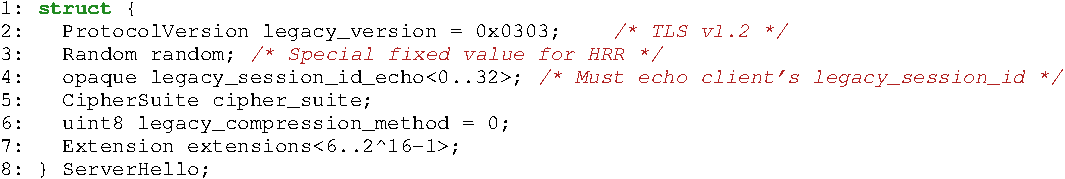
\includegraphics[width=.8\linewidth]{figure/ServerHello-struct.pdf}
    \captionsetup{width=.8\linewidth} 
    \caption[ServerHello and HelloRetryRequest Structures]{The structure of the ServerHello message, which is the same as the structure of HelloRetryRequest, repeated from Section 4.1.3 of \cite{esni} using the presentation syntax defined by same.}
    \label{lst:server-hello-struct}
\end{listing}

The use of the special constant value in the \var{random} field of the HRR has implications for the design of the ECH protocol. In the happy case when the server accepts the first \var{ClientHello} (it supports the cipher suites and the curves used for the \var{key\_share} etc.), and when the server also accepts ECH, then the last 8 octets of the \var{ServerHello.random} are filled with a special ECH acceptance signal. But in the case where HRR is necessary and ECH is accepted the last 8 octets of the \var{HRR.random} are not available because they are used to distinguish that the message is a HelloRetryRequest and not a ServerHello. Instead, in the case of HRR {\em and} ECH acceptance the ECH 8 byte acceptance signal is put in the \var{ECHClientHello.payload} field of an \var{encrypted\_client\_hello} extension (as described in Section 7.2.1 of \cite{esni}). Using a distinct extension to deliver stealthy ECH acceptance signal would not be acceptable because it would stick out.

Let's consider a TLS session in which a HRR is triggered. An easy way to achieve this practically is to set up a TLS 1.3 server which only supports an uncommon (EC)DHE group such as P-384. Most clients (including \var{openssl s\_client}) will not provide a P-384 \var{key\_share} by default in the ClientHello, and the server will respond with a HRR with a \var{key\_share} extension selecting \var{KeyShare.selected\_group = secp384r1}. Note that the server-to-client \var{key\_share} in a HRR message contains only an indication of the type of key share the server supports, but does not include a Key Share Entry. The total number of bytes in the \var{key\_share} extension in a HRR message is 6, 2 for the extension length, 2 for the extension type, and 2 for the Selected Group field. Therefore, there is no room in the HRR server-to-client \var{key\_share} to embed a stealthy ECH/SECH acceptance signal. The other extension that will be present in the HRR is the \var{supported\_versions}, which also has a length of 6 bytes, none of which can be manipulated stealthily.

Another option for sneaking an acceptance signal in the HRR could be to use the \var{cookie} extension as cover. The cookie extension (identified by \var{0x002C}) allows the server to send arbitrary data (of length \[1\] to \[2^{16}-1\] bytes) in either the HRR or the SH. In accordance with \var{rfc8446} when a client processes a cookie in an HRR it must echo the cookie extension exactly in in subsequent ClientHello2 message.

Since the cookie extension is allowed in HRR messages and can contain opaque data it can be used to send a secret acceptance signal. However, the cookie extension is not mandatory and may be used differently (or not used at all) by different servers. Thus, in order to successfully achieve a {\em stealthy} acceptance signal via the cookie, the extension would have to be manipulated in such a way that it does not stick out  when compared to normal TLS traffic. For instance the length of the cookie must not be an indicator of whether the cookie containts as acceptance signal. Also, if the cookie were to be used for the acceptance signal a censor could block all connections that use HRR cookies in order to thwart SECH.

\var{rfc8446} mention two purposes for the cookie extension;
\begin{enumerate}
    \item DoS mitigation: Forcing the client to echo back the cookie allows the server to verify that the client is `live', which increases the cost (and thus mitigates) DoS attacks.
    \item Offloading State: The cookie extension allows the server to `offload state' to the client, i.e. to ask the client to manage some data pertaining to the TLS connection. By offloading state to the client the server can determine which messages belong to the same connection while running statelessly.
\end{enumerate}

[ ] HRR Hijacking Explained

[ ] Risk of attacker using server as an oracle to reveal the inner SNI by forging a CH2.
        - For a design of a stealthy ECH protocol we require that the SECH acceptance signal also be stealthy. For ECH the acceptance signal is stealthy in the case that HRR is skipped, but it is not stealthy when HRR occurs. To facilate HRR while performing SECH we need a new mechanism to sneak the SECH acceptance signal to the client. One approach would be to delay the SECH acceptance signal until the true ServerHello, and put the SECH acceptance signal `ServerHello.random`. Another approach would be to use any other available random bytes in a typical HRR and replace them with the acceptance signal.

\subsection{Tickets and Session Resumption}

[ ] A TLS 1.3 server can issue tickets to clients after successful completion of a handshake. These tickets allow a client to initiate new TLS 1.3 sessions with the client in fewer steps (and with less computation) than is needed in the initial handshake.

The motivation for the TLS 1.3 ticket system comes from the typical behaviour of web browsers when loading and rendering web pages. Many contemporary web pages rely on a large number of resources to be loaded from the server. With the TLS ticketing system it is typical for a HTTPS server to issue several tickets (e.g. 6 or more) for every successful handshake. This means that when a web browser is loading a web page it can first complete a full handshake, and then open several more TLS connections to the server concurrently in order to load subsequent resources more quickly (e.g. images, videos, JavaScript files).

[ ] Details of tickets as specified by TLS 1.3 RFC. \var{psk\_binder}, \var{NewSessionTicket} message type, what happens when multiple servers have authority on the server's certificate?

[ ] the \var{pre\_shared\_key} extension
The structure of the \var{pre\_shared\_key} extension as defined in Section 4.2.11 of \cite{esni} is repeated in Listing \ref{lst:psk-struct}. When the client offers \var{pre\_shared\_key} it contains a list of (\var{identity}, \var{binder}) pairs, and if the server accepts PSK-based key establishment it sends back just the index of the selected identity. The \var{pre\_shared\_key} extension is exceptional because it
"MUST be the last extension in the ClientHello" (\citet[Section 4.2]{esni}). This restriction makes implementation of the \var{binders} slightly easier because the each binder in \var{binders} is a HMAC incorporating the entire \var{ClientHello} up to but excluding the list of \var{binders} themselevs.

The \var{PskIdentity} structure has an opaque \var{identity} field of between $1$ and $2^{16}-1$ bytes, which is plenty of room for stealthily sending encrypted data.

\begin{listing}
    \centering
    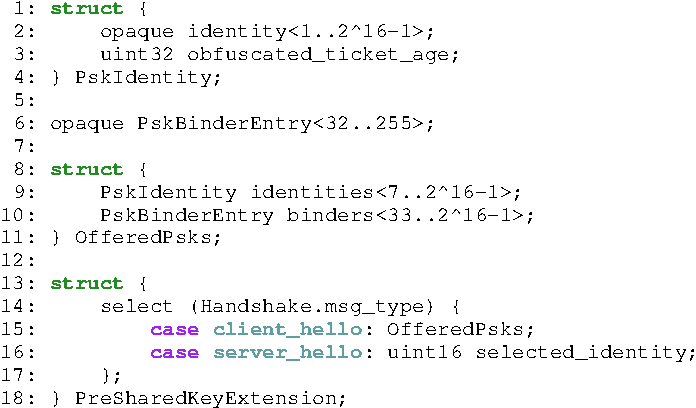
\includegraphics[width=.8\linewidth]{figure/pre_shared_key.pdf}
    \captionsetup{width=.8\linewidth} 
    \caption[Structures for the \var{pre\_shared\_key} extension]{TLS 1.3 presentation language representations of the structures used for the \var{pre\_shared\_key} extension.}
    \label{lst:psk-struct}
\end{listing}

[ ] Stateful/stateless cookies.

[ ] Notes about how tickets are typically used in reality. Notes about any strict restrictions on the ticket behaviour in TLS 1.3 RFC.

[ ] Introduce idea of using tickets to distribute access to an SECH server (will this be a way to distribute a symmetric key, or can the ticket allow a one-time connection that does not require the symmetric key?).

\subsection{ECH}

\subsubsection{ECHConfig}

% ECHConfig structure and fields
\cite{esni} define (in Section 4) just one version (identified by the hextet 0xfe0d) of the ECHConfig, but  the structure is defined in a way that will compatibly allow future versions. The interesting part of the ECHConfig is the ECHConfigContents which has four fields, the \var{key\_config}, the \var{maximum\_name\_length}, the \var{public\_name}, and \var{extensions}. The \var{key\_config} contains the \var{public\_key} needed by a client to encrypt the ClientHello under HPKE. As well as the \var{public\_key} the \var{key\_config} has a \var{config\_id}, a Key Encapsulation Method id (\var{kem\_id}) and a list of HPKE symmetric cipher suites supported by the ECHConfig. The \var{config\_id} is ``A one-byte identifier for the given HPKE [public] key''.

% hard to send config\_id stealthily
When a client offers ECH it sends the \var{config\_id} of the public key used to encrypt the ClientHelloInner. This \var{config\_id} means that the server only has to attempt decryption of the ClientHelloInner once, which is essential for a scalable deployment of ECH. In the case of a stealthy ECH variant, however, transmitting a \var{config\_id} stealthily in the first flight of messages from the client (without permitting an attacker to detect the SECH \var{config\_id}) is a non-trivial challenge.

[ ] Distributing Access to Backend Servers: (for TLS 1.3 the client just needs the servername and IP address, but for ECH the client additionally needs the public key of the ECH backend server). The ECHConfig will typically be distributed using DNS, which means that the ECH backend server will be advertising its own existence to users and censors alike. But other ways of distributing ECH configurations (which a client needs to establish a connection to a backend ECH server), such as having the ECH config preconfigured in the client, are also permissable.

[ ] Considering that the ECH protocol is not stealthy there is little harm done in advertising the existence of the ECH backend server, it would be possible for a powerful attacker to enumerate backend servers with high confidence using DPI and traffic analysis.

[ ] For SECH we have an opportunity to hide the existence of backend SECH servers from attackers, which may be particularly beneficial for censorship-circumvention use cases. If the existence of the backend SECH server can be hidden from potential censors then the censor will not be motivated to (over)block access to the SECH facilitating client-facing server. More on this later.

\subsubsection{How ECH mitigates cut-and-paste attacks}
Here we examine the mechanism used in the current draft of ECH to mitigate cut-and-paste attacks. A cut-and-paste attack against a servername encryption protocol could be used by an attacker to unveil the intended backend server of a connection as described in Section 3.1 of \cite{rfc8744-issues}. The following description of how a cut-and-paste attack could leak a cut-and-paste attack is after \cite{rfc8744-issues}.
\begin{enumerate}
    \item A benign client sends a ClientHello with an encrypted SNI included.
    \item An attacker copies the encrypted SNI into a new ClientHello.
    \item The client-facing/backend servers have no mitigation against the replay of the encrypted SNI and establish a connection between the attacker and backend server.
    \item To conclude the handshake the backend server sends \var{Certificate} and \var{CertificateVerify} messages, revealing the identity of the backend server that the benign client intended to reach. 
\end{enumerate}
\cite{esni} note in Section 10.10.1 that a cut-and-paste attack is not possible against ECH because a server either processes a \var{ClientHelloOuter} or \var{ClientHelloInner} and \var{ClientHelloInner.random} is encrypted. Since \var{ClientHelloInner.random} is encrypted using a public key from an ECHConfig, only the client (who encrypted it) and the possessor of the corresponding private key can view \var{ClientHelloInner.random}. Therefore, if a malicious client tries to replay an \var{encrypted\_client\_hello} extension, it will contain a \var{ClientHelloInner.random} value that has already been used.

To understand why ECH doesn't leak the inner SNI in the case of a cut-and-paste attack, let's look at how the attack would play out:
\begin{enumerate}
    \item A client sends a \var{ClientHelloOuter} with an encrypted \var{ClientHelloInner}.
    \item Attacker cuts and pastes the entire ClientHelloOuter (cannot cut-and-paste just the \var{encrypted\_client\_hello} extension because the encrypted payload is cryptographically bound to the ClientHelloOuter).
    \item The client-facing server successfully decrypts the replayed \var{encrypted\_client\_hello} payload and forwards ClientHelloInner to the backend server. (A sophisticated backend server could reject the repeated ClientHelloInner.random, but that is not sufficient to stop the attack [1]).
    \item The backend server accepts ECH (but the attacker cannot verify acceptance because it doesn't have the plain-text ClientHelloInner necessary for \var{transcript\_ech\_conf}, which is in turn necessary for \var{accept\_confirmation}).
    \item Backend server sends \var{ServerHello}, \var{\{Certificate\}}, \var{\{CertificateVerify\}}.
    \item However, {Certificate} is protected with \var{\shts} which can only be derived if the full ClientHelloInner is known. While much of \var{ClientHelloInner} could be guessed by an attacker with reasonable probability, the \var{ClientHelloInner.\-random} can only be guessed with probability $1/2^{256}$ (32 octets). Also, the \var{\shts} is derived from the (EC)DHE handshake, but whether using a \var{key\_share} or a PSK the attacker cannot complete the DH exchange because it doesn't know the private values associated with \var{key\_share}, nor the \var{key\_share} which is encrypted in the \var{ClientHelloInner} (same for PSK).
\end{enumerate}


In summary, an attacker can trigger a backend server to send an encrypted {Certificate}, but cannot decrypt the {Certificate}.


% CLIENT                            CF-SERVER                             BACKEND SERVER
% ClientHelloOuter
% +encrypted\_client\_hello
% --------------------------------------->
%                                          ClientHelloInner
%                                          ------------------------------->
%                                                               ServerHello
%                                                      +accept\_confirmation
%                                          <-------------------------------
%                              ServerHello
%                     +accept\_confirmation
% <---------------------------------------

\subsubsection{ECH acceptance}

[ ] As noted above the ECH acceptance signal is embedded into the first message sent by the server, whether the first message is a ServerHello or a HelloRetryRequest, however the location of the message is different in the HRR. This difference is an unfortunate added complexity. An alternative design might have had the ECH acceptance signal always embedded in the ServerHello, whether or not a HRR is issued. The reason such a design would not be acceptable is that the client needs to know whether a message it is processing was constructed by the client-facing server or the backend server, including whether the HRR was sent by the client-facing or backend server. If the HRR is constructed by the client-facing server (i.e. ECH was rejected), then the HRR corresponds to the ClientHelloOuter, but if the HRR was constructed by the backend server then it corresponds to the ClientHelloInner. In order for the client to construct a valid CH2 it needs to know which ClientHello message the HRR is rejecting.  While it may have been possible for a client to infer from the HRR contents (without an ECH acceptance signal) which ClientHello message it corresponds to (e.g. by process of elimination on the supplied cipher suites in either CH), this approach would not be robust and would make extensions to the protocol more complicated yet. Also, without the ECH acceptance signal it may be more difficult to analyse the security properties of the protocol due to an increased number of possible states the client can be in after processing the HRR.
Also, according to \cite{esni} when a client offers ECH but the server does not accept then the client must terminate the connection with a \var{ech\_required} alert, which is not encrypted and thus transparent to network observers. In order to reduce the amount of unnecessary traffic ECH is designed so that the client can decide whether to emit the terminal \var{ech\_required} alert upon receipt of first server message. A stealthy variant of ECH should not conspicuously terminate the connection when SECH is rejected, but ought to either continue with the handshake or emit an inconspicuous alert in order to conceal the fact that SECH was attempted.

\includefigure{fig:ech-reject-and-hrr}{Sequence Diagram of ECH Rejection and HRR}{A sequence diagram for a session in which the client attempts ECH but ECH is rejected {\em and} the parameters of the ClientHelloOuter aren't supported (hence HRR). Since ECH is rejected the client responds with a fatal \var{ech\_required} alert in compliance with Section 5 of \cite{esni}}{figure/ech-reject-and-hrr.pdf}


\section{Considering a stealthy variant of ECH}
\subsection{Finding cover in TLS 1.3}
[ ] we can find cover by using any parts of the TLS 1.3 client messages that look (or are) random
[ ] \var{ClientHello.random}
[ ] \var{ClientHello.legacy\_session\_id}
\subsection{Offering Both ECH and SECH}
While it is not immediately obvious that offering **both** ECH and a stealthy SECH variant could be beneficial there are some circumstances where offering both may in the future be necessary to protect privacy or facilitate censorship circumvention. In particular the risk that ECH will be blocked outright by some powerful censors (e.g. in China), means that the convenience and enhanced privacy of regular ECH may be preferable in regions where ECH is not blocked, but the stealthy alternative may be the only way to access the domain privately from regions where ECH is blocked. This is a clear case where domains may in future wish to offer both ECH and SECH.

But offering thes two methods for accessing a resource privately is an inherent increase in complexity of the overall system compared to a system that only offers *either* ECH *or* SECH. This increase in complexity increases the attack surface of the system, there will be more branches of code on both the client and the server, the cost of developing and deploying the additional code will be significant, and the simultaneously co-operability of the two protocols presents new challenges to the design of each. That the two protocols should co-operate also introduces an additional burden of analysis in terms of identifying and mitigating attacks against each of the protocols. For all of these reasons there is a strong temptation to pursue developing versions of ECH and SECH that are designed *not* to co-operate with each other. However, another pattern of argument relevant to most security protocols emphasises the importance of having a stand-by backup option to a widely deployed algorithm. For instance, the most popular/widely-deployed AEAD algorithm on the internet is AES-128-GCM, but many software packages also support ChaCha20-Poly1305 because it could transpire at any moment that AES-128-GCM has a fundamental flaw and needs to be replaced urgently. This argument can also be applied to ECH and SECH; it would be wise to have both options ready, well-analysed, and deployed such that either one can be quickly disabled in case a fatal security flaw is discovered.

The above argument pertains to the simultaneous deployment of ECH and SECH for a single domain, but what about having versions of SECH and ECH that facilitate the server accepting both ECH and SECH within a single TLS session? Is there a motivation for such a design? Consider, for example, an enterprise network in which the enterprise has control of client devices and is able to manage the list of trusted CAs on each client device. In such a case the enterprise network administrator will be able to mount a MITM attack, which would allow inspection of the TLS 1.3 application traffic as well as the encrypted ClientHello if ECH is being used. There is motivation for network administrators to enforce such a situation for various reasons, e.g. the enterprise network may be attempting to thwart phishing campaigns, and the risks of phishing campaigns can be mitigated by blocking traffic to suspicious or known malevolent domain names. We can foresee a scenario, then, where the network administrator decides to mount a MITM attack in order to inspect the encrypted ClientHello, but no other part of the TLS 1.3 encrypted traffic. Let's imagine now we have a client trying to circumvent this MITM attack. If ECH is available and used by default then it would be suspicious for the client not to use ECH. However, the client may observe that using ECH to connect to `blocked.example.com` gets blocked, and therefore will have to access `blocked.example.com` by some other means. In such a case the client would benefit from the ability to make a 'cover' ECH connection request (to `allowed.example.com`, say) and simultaneously an SECH connection request to `blocked.example.com`. To accomodate this scenario we would like for it to be possible to attempt ECH and SECH on the same connection.

It seems unlikely, however, that there would be much benefit from the server being able to accept both ECH and SECH, since the acceptance signal for ECH is sent in the same flight as the server certificate. If ECH and SECH are both accepted by the server, but with differing inner servernames (e.g. `ech.example.com` and `sech.example.com`), the server will have to select a certificate to send for the same flight of messages as the ECH acceptance signal. Possibly, it would be beneficial to the client to know that both were accepted, such that it can decide how to try to establish subsequent connections. 

\subsection{Accepting SECH}

[ ]  The ECH acceptance signal is necessary because the client continues the handshake differently (e.g. the Finished message is constructed with a transcript using the ClientHelloInner) when it detects a positive ECH \var{accept\_confirmation} signal from the server. The design of the ECH acceptance signal facilitates ECH split-mode, in which the backend server only processes one ClientHello (ClientHelloInner if the client-facing server accepts ECH, and ClientHelloOuter otherwise).

[ ] The purpose of an SECH acceptance signal is to inform the client as early as possible whether or not the server is intending to use the inner or outer servername. It is sufficient to include only a positive signal (the server is accepting the SECH inner servername), and to infer that the outer servername will be used when the positive signal is absent.
    - Detecting the length of the domain name

[ ] must not be possible for an attacker to detect the length of the inner servername, merely knowing the length of the servername could leak the servername itself
